\subsubsection{Background}
Simulating molecule system with high accuracy in VQE is both a time and memory consuming task. The memory used to simulate hydrogen chains in different sizes is shown in table~\ref{tab:memory_h_chain}

\begin{table}[ht]
    \begin{tabular}{ccc}
        \toprule
        Hydrogen chain & Qubit Number & Memory with Complex128 \\
        \midrule
        $H_2$          & 4            & 0.256kB                \\
        $H_6$          & 12           & 64kB                   \\
        $H_{10}$       & 20           & 16MB                   \\
        $H_{14}$       & 28           & 4GB                    \\
        $H_{18}$       & 36           & 1TB                    \\
        \bottomrule
    \end{tabular}
    \caption{Memory consumption for storing full amplitudes quantum state.}
    \label{tab:memory_h_chain}
\end{table}

Based on UCCSD (Unitary coupled-cluster with singles and doubles) theory, the ansatz is described as:
\begin{equation}
    |\Psi(\vec{\theta})\rangle = e^{(\hat{T}-\hat{T}^\dagger)}\ket{\psi_\text{HF}},
\end{equation}
where $\hat{T}$ is couple cluster operator, and $\ket{\psi_\text{HF}}$ is Hartree-Fork state. The couple cluster operator is written as:
\begin{equation}
    \hat{T}=\sum_{p\notin\text{occ},q\in\text{occ}}\theta_q^p \hat{a}_p^\dagger \hat{a}_q + \sum_{pq\notin\text{occ},rs\in\text{occ}}\theta_{rs}^{pq}\hat{a}_p^\dagger \hat{a}_q^\dagger \hat{a}_r \hat{a}_s,
\end{equation}
and under one order trotterization the ansatz can be decomposed to:
\begin{equation}
    |\Psi(\vec{\theta})\rangle\approx \prod_ie^{(\hat{T}_i-\hat{T}_i^\dagger)}\ket{\psi_\text{HF}}.
\end{equation}
Taking hydrogen chain $H_6$ for example, we need 12 qubits to simulate this system and there are 6 electrons with 3 spin up and 3 spin down. Fig.~\ref{6_1_h6_a} shows the Hartree-Fork state of $H_6$ and Fig.~\ref{6_1_h6_b} shows the spin-orbital under excitation operator $\hat{T}=\hat{a}_{11}^\dagger \hat{a}_{10}^\dagger \hat{a}_5 \hat{a}_4$.
\begin{figure}
    \centering
    \begin{subfigure}{0.3\textwidth}
        \centering
        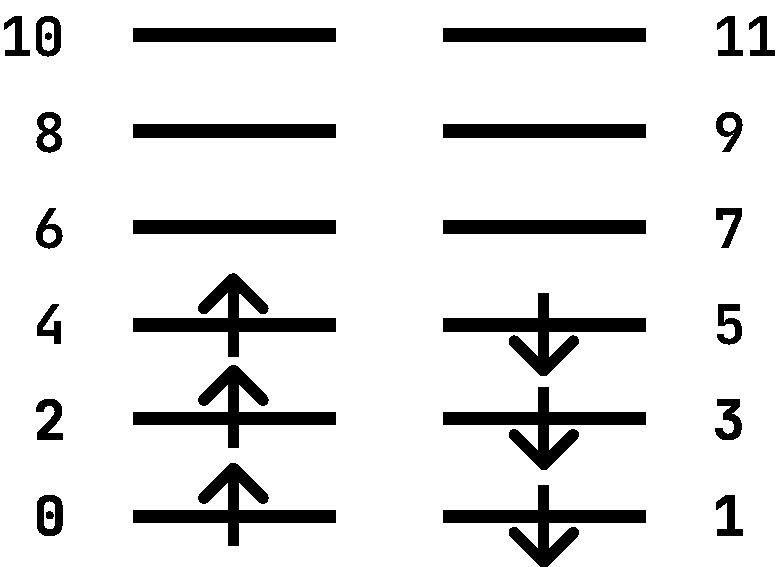
\includegraphics[width=\textwidth]{images/6_1_h6_a.pdf}
        \caption{Hartree-Fork state of $H_6$.}
        \label{6_1_h6_a}
    \end{subfigure}
    \begin{subfigure}{0.3\textwidth}
        \centering
        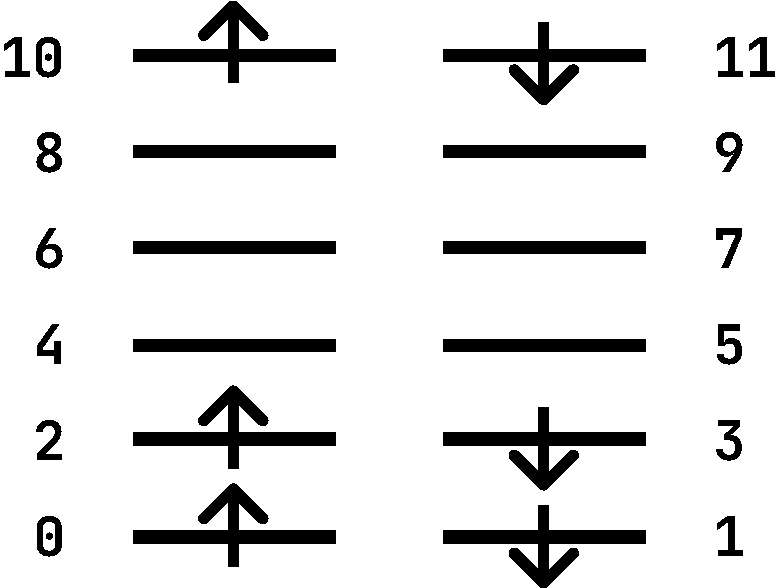
\includegraphics[width=0.9\textwidth]{images/6_1_h6_b.pdf}
        \caption{Spin-orbital after applying excitation operator $\hat{T}=\hat{a}_{11}^\dagger \hat{a}_{10}^\dagger \hat{a}_5 \hat{a}_4$.}
        \label{6_1_h6_b}
    \end{subfigure}
\end{figure}
\subsubsection{Electron and spin conservation}
In \QuPack, we impose the constraint that the total number of electrons and the total spin number of electrons remain constant throughout the evolution of the ansatz. This constraint significantly reduces the dimension of the Hilbert space that we need to simulate. Suppose the qubit number is $n_q$ and the electron number is $n_e$, the dimension of full amplitude state is $2^{n_q}$, but after electron and spin conservation, the dimension will be:
\begin{equation}
    \binom{n_q/2}{n_e/2}^2=\left(\frac{(n_q/2)!}{(n_e/2)!(n_q/2-n_e/2)!}\right)^2.
\end{equation}
The memory consumption will reduce from 1TB to $\sim$35GB.

Besides the memory reduction, we also optimized the evolution of coupled cluster operator. For a given coupled cluster operator $\hat{V}(\theta)=e^{\theta(\hat{T}-\hat{T}^\dagger)}$, it is easy to prove that $(\hat{T}-\hat{T}^\dagger)^3 = - (\hat{T}-\hat{T}^\dagger)$ and $(\hat{T}-\hat{T}^\dagger)^4 = -(\hat{T}-\hat{T}^\dagger)^2$. After Taylor expansion, we have:
\begin{equation}
    \hat{V}(\theta) = \mathbb{I} + ( 1-\cos\theta)(\hat{T}-\hat{T}^\dagger)^2 + \sin\theta (\hat{T}-\hat{T}^\dagger).
\end{equation}
Choose a calculation base in reduced Hilbert space $\ket{i}$, so that $\hat{T}\ket{i} = \ket{j}\neq0$, then we have $\hat{T}^\dagger\ket{i}=0$ and $\hat{T}^\dagger\ket{j}=\ket{i}$. The evolution of coupled cluster can be simplified to:
\begin{equation}
    e^{\theta(\hat{T}-\hat{T}^\dagger)}\begin{pmatrix}
        \ket{i} \\\ket{j}
    \end{pmatrix}=\begin{pmatrix}
        \cos\theta  & \sin\theta \\
        -\sin\theta & \cos\theta
    \end{pmatrix}\begin{pmatrix}
        \ket{i} \\\ket{j}
    \end{pmatrix}.
\end{equation}
And for $e^{i\theta(\hat{T}+\hat{T}^\dagger)}$, we have
\begin{equation}
    e^{i\theta(\hat{T}+\hat{T}^\dagger)}\begin{pmatrix}
        \ket{i} \\\ket{j}
    \end{pmatrix}=\begin{pmatrix}
        \cos\theta   & i\sin\theta \\
        -i\sin\theta & \cos\theta
    \end{pmatrix}\begin{pmatrix}
        \ket{i} \\\ket{j}
    \end{pmatrix}.
\end{equation}

When doing variational quantum algorithm on this system, we need to calculate the gradient of $\hat{V}(\theta)$, which is given as:
\begin{equation}
    \frac{\partial \hat{V}(\theta)}{\partial\theta}\begin{pmatrix}
        \ket{i} \\\ket{j}
    \end{pmatrix}=\begin{pmatrix}
        -\sin\theta & \cos\theta  \\
        -\cos\theta & -\sin\theta
    \end{pmatrix}\begin{pmatrix}
        \ket{i} \\\ket{j}
    \end{pmatrix}.
\end{equation}

Here is a demonstration code of how to build a quantum circuit of evolution of coupled cluster operator.

\begin{lstlisting}
from qupack.vqe import ExpExciteGate
from mindquantum.algorithm.nisq import uccsd_singlet_generator
from mindquantum.core.circuit import Circuit

ucc_fermion_ops = uccsd_singlet_generator(6, 4)
circ = Circuit()
for term in ucc_fermion_ops:
    circ += ExpExciteGate(term)
\end{lstlisting}

A specific simulator, known as \code{ESConservation}, has been designed to efficiently simulate the coupled cluster operators within a subspace of the Hilbert space. This specialized simulator, which shares the same API as the simulator in \MindQuantum, excels in accurately modeling the intricate dynamics of these operators.
